\chapter{Abstandsautomaten}\label{Abstandsautomaten}
Diese Kapitel beschreibt die theoretischen Ergebnisse in Bezug auf die Abstandsautomaten. Das Muster sei dabei der \glqq fehlerfreie\grqq Text, mit dem eine Eingabe verglichen werden soll.
\section{Spezielle Abstandsautomaten}
Der \textbf{Abstand} oder die \textbf{Distanz} zwischen zwei Wörtern ist definiert als die minimale Anzahl an Operationen, die benötigt werden, um ein Wort in das andere zu überführen. Welche Operationen dabei erlaubt sind, hängt von dem Abstand ab. Abstände sind Metriken auf dem Raum von Symbolsequenzen. Eine Metrik ist eine Funktion, die jedem Paar von Elementen des Raums einen nicht negativen reellen Wert zuordnet. Metriken sind definit, symmetrisch und erfüllen die Dreiecksungleichung.
\subsection{Hamming-Abstand}
Beim Hamming-Abstand ist nur Substitution von Buchstaben erlaubt. Das bedeutet insbesondere, dass Muster und Eingabe die gleiche Länge haben müssen.

\begin{figure}[!htb]
\centering
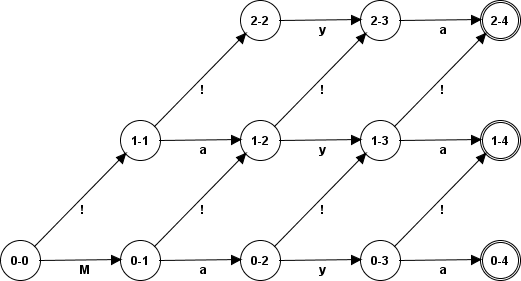
\includegraphics[scale=0.7]{pic/automata/hamming}%
\caption{Ein Hamming-Automat mit dem Abstand 2 für das Muster Maya}%
\end{figure}
Die unterste Zeile ist die Zeile ohne Fehler, jeweils eine Zeile höher bedeutet ein Fehler mehr. Die Anzahl der Zeilen entspricht also dem Abstand + 1. Mit jedem Buchstaben der Eingabe wandert man eine Spalte nach rechts. Ein waagerechter Else-Übergang bedeutet ein zum Muster passender Buchstabe, ein diagonaler ein nicht passender.
\subsection{Levenshtein-Abstand}
Der Levenshtein-Abstand erlaubt zusätzlich zur Substitution von Buchstaben auch das Einfügen und Löschen von Buchstaben.

\begin{figure}[!htb]
\centering
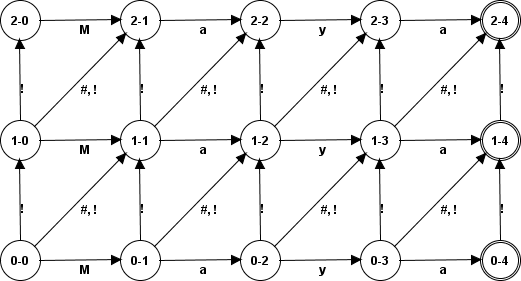
\includegraphics[scale=0.7]{pic/automata/levenshtein}%
\caption{Ein Levenshtein-Automat mit dem Abstand 2 für das Muster Maya}%
\end{figure}
Der Grundaufbau ist derselbe wie bei dem Hamming-Automaten. Es kommen lediglich zwei Übergangstypen hinzu. Ein senkrechter Else-Übergänge bedeutet ein Einfügen eines Buchstabens, ein diagonaler spontaner Übergänge das Löschen eines Buchstabens.

\subsection{Damerau-Levenshtein}
Der Damerau-Levenshtein-Abstand erlaubt neben der Substitution auch das Einfügen und Löschen von Buchstaben Transposition benachbarter Buchstaben. In der Praxis ist dies relevant, da Vertauschen benachbarter Buchstaben ein typischer Tippfehler ist. Sowohl Substitution als auch Transposition könnte durch zwei Operationen (Einfügen und Löschen) erreicht werden. Jedoch führt dies zu einem anderen Abstand.
\section{Motivation universeller Automaten}
Anwendungsgebiet von Abstandsautomaten ist z.B. die Rechtschreibkorrektur, wobei ein Wort, dass nicht im Wörterbuch gefunden wird mit einem bestimmten Abstand auf jedes Wort im Wörterbuch getestet wird. Die akzeptierten Wörter bilden dann die Menge der Korrekturvorschläge. Andere Anwendungen wären z.B. alternative Suchvorschläge (\glqq Meinten Sie ...\grqq) oder bei fehlerbehafteter Datenübertragung.

Der Test des Abstandes muss oft sehr schnell gehen, da sehr viele Tests durchgeführt werden sollen. Während der Automat für Hamming deterministisch ist, gilt dies nicht für Levenshtein- und Damerau-Levenshtein-Automaten (Problem ist die Entscheidung welche Operation benutzt werden soll). Simulation von Nichtdeterminismus bedeutet einen deutlich größeren Aufwand. Auch das Umwandeln der NEAs in äquivalente DEAs durch Potenzmengenkonstruktion ist relativ aufwändig und die resultierenden Automaten wären sehr groß (Abhängig von der Länge des Musters).

Dadurch ist die Idee motiviert, universelle Abstandsautomaten einzuführen. Dabei muss nur ein einziges mal (für einen festen Abstand) der Automat konstruiert werden (und ggf. deterministisch gemacht werden). Der Preis dafür ist eine notwendige Kodierung der Eingabe vor der Simulation.

Die Idee eines universellen Levenshteinautomaten wurde in \cite{lit01} vorgestellt. Ziel dieser Arbeit ist es, die dort vorgestellte Form des Automaten zu untersuchen und Funktionsweise und Konstruktion zu erläutern. Außerdem sollen universelle Abstands-Automaten auch für den (einfacheren) Hamming-Abstand und den (komplizierteren) Damerau-Levenshtein-Abstand untersucht werden.
\section{Ergebnisse}
\subsection{Hamming-Abstand}
\begin{figure}[!htb]
\centering
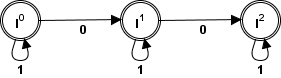
\includegraphics[scale=0.7]{pic/automata/unihamming}%
\caption{Ein universeller Hamming-Automat mit dem Abstand 2}%
\end{figure}
Ein universeller Abstandsautomat für den Hamming-Abstand ist durchaus möglich, aber überflüssig. Zum einen ist der spezielle Hamming-Automat bereits deterministisch. Außerdem ist der Aufwand zu Kodierung der Eingabe bereits mindestens so groß wie die Berechnung des Abstandes selbst. Da beim Hamming-Abstand nur Substitution erlaubt ist, reicht es zur Berechnung des Abstandes, jeden i-ten Buchstaben auf Gleichheit zu testen und bei jeder Ungleichheit den Abstand um 1 zu erhöhen. Dieser Vergleich muss beim Kodieren der Eingabe ebenfalls geschehen und entsprechend als 0 im Falle der Ungleichheit und 1 im Falle der Gleichheit an der i-ten Stelle in der codierten Eingabe auftauchen. Der Fall der ungleichen Längen muss gesondert behandelt werden, da in diesem Fall der Abstand nicht definiert ist. Die kodierte Eingabe könnte in diesem Fall aus einem Dummy-Symbol bestehen oder eines oder mehrere Dummy-Symbole beinhalten, die keinen Übergang im Automaten haben.
\subsection{Levenshtein-Abstand}
\begin{figure}[!htb]
\centering
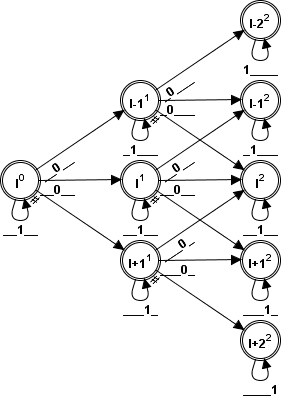
\includegraphics[scale=0.7]{pic/automata/unilevenshtein}%
\caption{Ein universeller Levenshtein-Automat mit dem Abstand 2}%
\end{figure}
Die Idee beim universellen Automaten für den Levenshtein-Abstand ist, dass in jedem Schritt die gleiche Entscheidung getroffen werden muss, nämlich ob ein passender, ein löschender, ein einfügender oder ein substituierender Schritt gemacht werden soll. Die einzigen Vorinformationen, die benötigt werden, sind, wieviele Fehler bereits gemacht wurden und mit dem wievielten Buchstaben des Musters verglichen werden muss. Das ist notwendig, denn die Zahl der Berechnungsschritte lässt sich nicht eins zu eins auf die Buchstaben des Musters abbilden. Wurde ein Buchstabe gelöscht, muss ein Buchstabe weiter vorne im Muster abgeglichen werden. Wurde ein Buchstabe eingefügt, muss ein Buchstabe weiter hinten abgeglichen werden. Substitution und passende Übergänge ändern dies nicht. Die Anzahl der Fehler lassen sich leicht im Zustand kodieren. Allerdings muss in jedem Zustand der Vergleich zu jedem möglichen Musterbuchstaben (beschränkt durch den Abstand) zur Verfügung stehen. Welcher Vergleich betrachtet wird, wird wieder im Zustand kodiert.

\begin{figure}[!htbp]
\centering
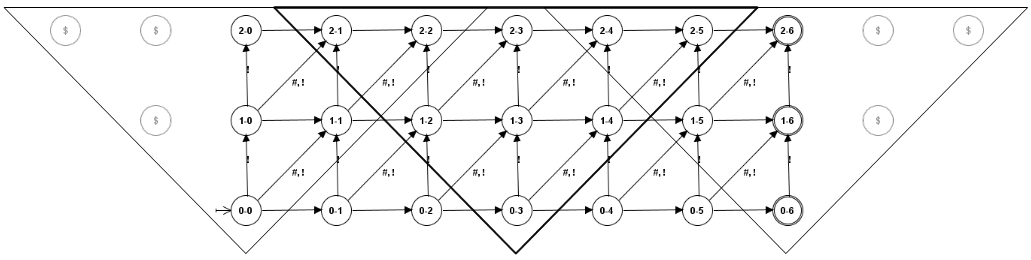
\includegraphics[width=\linewidth,height=\textheight,keepaspectratio]{pic/dreiecke2}%
\caption{Symbolische Dreiecke - erreichbare Zustände nach n verarbeiteten Buchstaben}%
\end{figure}
Betrachtet man die erreichbaren Zustände nach n verarbeiteten Buchstaben der Eingabe im speziellen Automaten liefert das ein gleichschenkliges Dreick mit der Spitze unten (vgl. Bild). Dies sind die Zustände, die im universellen Automaten vorkommen. Damit für den Beginn und das Ende, wenn die Dreicke nicht mehr vollständig sind, keine gesonderte Behandlung erfolgen muss, werden einfach virtuelle Zustände an den fehlenden Stellen angenommen. Dies findet sich auch in der Kodierung wieder.

Die Kodierung muss also für jeden Berechnungsschritt einen Block der Größe $2*k+1$ liefern, wobei $k$ der Abstand ist. Dieser Block wird in Mihov/Schulz charakteristischer Vektor genannt. Jedes Zeichen des charakteristischen Vektors ist entweder eine 0 oder eine 1, je nachdem ob der Buchstabe der Eingabe mit dem entsprechenden Buchstaben des Teils des Musters übereinstimmt. Da bei Beginn der Simulation kein Fehler gemacht wurde, ist zunächst der mittlere Buchstabe relevant, deshalb muss der erste Teil der Musters in der Mitte beginnen und die ersten k Symbole sind 0 (werden z.B. mit einem Buchstaben verglichen, der im Alphabet nicht vorkommt, vergleiche virtuelle Zustände im oben beschriebenen symbolischen Dreieck). In jedem Schritt wird der Vergleichsblock um 1 nach links geshiftet und mit dem nächsten Buchstaben aus dem Muster aufgefüllt. Ist das Muster zu Ende, werden wie am Anfang Dummy-Buchstaben eingefügt. Es müssen so viele charakteristische Vektoren erzeugt werden, bis die Eingabe zu Ende ist und das letzte Zeichen des Musters an erster Stelle im Vergleichsblock ist. All diese charakteristischen Blöcke werden dann konkateniert und bilden die tatsächliche Eingabe zur Simulation.\\
\begin{table}[!htbp]
\begin{longtable}{c|c||c}
Eingabesymbol & Vergleichsblock & kodierter Block/""charakteristischer Vektor \\ \hline \endhead
M & \$\$May & 00100 \\
a & \$Maya & 00101 \\ 
j & Maya\$ & 00000 \\
a & aya\$\$ & 10100 \\
h & ya\$\$\$ & 00000 \\
\$ & a\$\$\$\$ & 01111 \\
\end{longtable}
\caption{Beispiel: Eingabe Majah bei dem Muster Maya für den Abstand 2.}
\end{table}

Die signifikante Stelle eines Zustandes sei Stelle Mitte + Löschvorgänge - Einfügevorgänge. Unabhängig von der Fehleranzahl gibt es in jedem Zustand eine Schleife mit einer 1 an der signifikanten Stelle, die restlichen Stellen spielen keine Rolle (dürfen also 0 oder 1 sein). Diese Schleife repräsentiert der Fall, dass kein Fehler an dieser Stelle gemacht werden muss. Für den Fehlerfall gibt es drei Übergänge zu den erreichbaren Zuständen der nächsten Fehlerstufe. Für einen Einfügevorgang und einen Substitutionsvorgang hat der Übergang an der signifikanten Stelle eine 0, wobei die anderen Zeichen wieder keine Rolle spielen. Es ist ebenso möglich, an der Stelle auch eine 1 zu akzeptieren, in diesem Fall wird der Automat allerdings nicht minimal (und der Potenzmengenautomat wird auch größer). Der Löschvorgang hat die Besonderheit, dass der soeben verarbeitete Buchstabe anschließend noch verglichen werden muss. Dafür gibt es zwei Möglichkeiten. Zum einen kann der Übergang mit einer 0 an der signifikanten Stelle und einer 1 an der signifikanten Stelle + 1 erfolgen. Dies deckt jedoch nicht den Fall ab, dass mehrere Löschvorgänge hintereinander gemacht werden können. Dafür werden zusätzliche Kanten in die höheren Fehlerstufen benötigt mit 0 an der signifikanten Stelle des Startzustandes und einer 1 an der signifikanten Stelle des Zielzustandes. Die Alternative ist, diesen Übergang spontan zu machen, was aber bedeutet diesen Übergang auch bei einem fehlerlosen Übergang zu ermöglichen, wodurch -- wie oben -- ein größerer Automat entsteht.

Der Startzustand ist der einzige Zustand in der fehlerfreien Stufe. Alle Zustände sind Endzustände. Die Erkennung des Endes der Eingabe wird durch die Kodierung des Wortes abgedeckt. Dieser NEA kann dann durch Potenzmengenkonstruktion in einen DEA umgewandelt werden.

\begin{figure}[htbp]
\centering
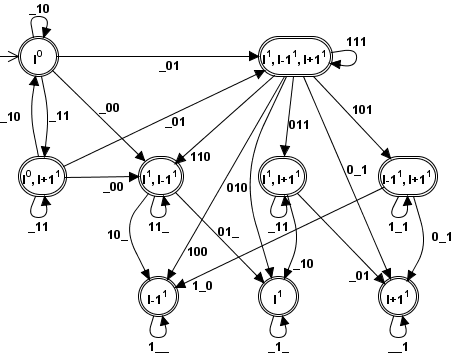
\includegraphics[scale=0.7]{pic/automata/unidlevenshteina}%
\caption{Die deterministische Version des Levenshtein-Automaten für den Abstand 1}%
\end{figure}
\begin{figure}[htbp]
\centering
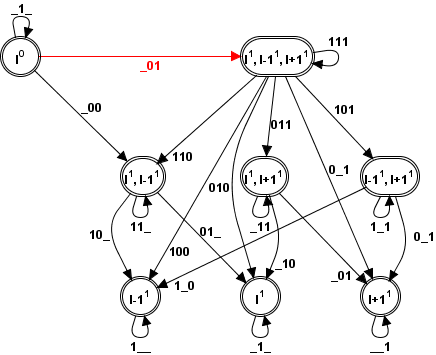
\includegraphics[scale=0.7]{pic/automata/unidlevenshteinb}%
\caption{Die deterministische Version des Levenshtein-Automaten für den Abstand 1 mit geforderter 0 bzw. die minimierte Version.}%
\end{figure}
\subsection{Damerau-Levenshtein}
Ausgegangen wird von dem universellen Levenshtein-Automaten aus dem letzten Abschnitt. Die Kodierung der Eingabe ist dieselbe.

Für jeden Zustand in allen Fehlerstufen außer der letzten, wird ein zusätzlicher Zwischenzustand benötigt. Dieser ist dadurch motivert, dass eine Transposition zwei Vergleiche benötigt, um erkannt zu werden. Der Tausch eines Zeichens von hinten nach vorne und umgekehrt ist äquivalent, es muss also nur ein Fall behandelt werden. Von dem Ursprungszustand zu diesem Zwischenzustand geht also ein Übergang mit einer 0 an der signifikanten Stelle des Zustandes und einer 1 an der signifikanten Stelle + 1. Von diesem Zwischenzustand geht ein Übergang mit einer 1 an der signifikanten Stelle - 1 zu dem Zustand mit derselben signifikanten Stelle in der nächsten Fehlerstufe.

Diese Übergänge sind in der Lage, einfache, unabhängige Tauschoperationen zu erkennen. Mehrfach verknüpfte Tauschoperationen oder Tauschoperationen in Verbindung mit Einfüge- oder Löschoperationen werden dadurch nicht erkannt. Eine Tauschoperation mit einem Substitutionsvorgang verknüpft, ergibt keinen Sinn. Außerdem müssen Tauschoperationen, bei denen ein bereits getauschter mit einem nicht getauschten Buchstaben vertauscht werden (also das \glqq Durchreichen\grqq eines Buchstabens), nicht gesondert betrachtet werden. Dieser Effekt kann ab zwei Tauschoperationen mindestens mit genauso wenig Operationen erreicht werden, indem das Symbol an der \glqq falschen\grqq Stelle gelöscht und an der \glqq richtigen\grqq Stelle eingefügt wird (konstant zwei Operationen).

Betrachtet man Tauschvorgänge von jeweils bereits unabhängig getauschten Symbolen (relevant ab einem Abstand von 3), lässt sich feststellen, dass der gleiche Effekt durch eine Tauschoperation verknüpft mit einem Lösch- oder Einfügevorgang erreicht werden kann. Folgende Beispiele machen dies deutlich:\\
$
abcd \rightarrow bacd \rightarrow badc \rightarrow bdac\\ \text{\quad 3 Tauschoperationen}\\
abcd \rightarrow bacd \rightarrow bdacd \rightarrow bdac\\ \text{\quad 3 Operationen: 1 Tausch mit 1 Einfügevorgang, 1 Löschvorgang}\\
%\end{align}
%\begin{align}
abcde \rightarrow bacde \rightarrow badce \rightarrow bdace \rightarrow bdaec\\ \text{\quad 4 Tauschoperationen}\\
abcde \rightarrow bacde \rightarrow bdacde \rightarrow bdace \rightarrow bdaec\\ \text{\quad 4 Operationen: 1 Tausch mit 1 Einfügevorgang, 1 Tausch mit 1 Löschvorgang}
$%\end{align}

Die benötigten Übergänge für die Einfüge- und Löschvorgänge werden analog zu denen im Levenshtein-Automaten eingefügt. Diese Übergänge sind notwendig; ob sie hinreichend sind, ist noch nicht abschließend untersucht.

\begin{figure}[htbp]
\centering
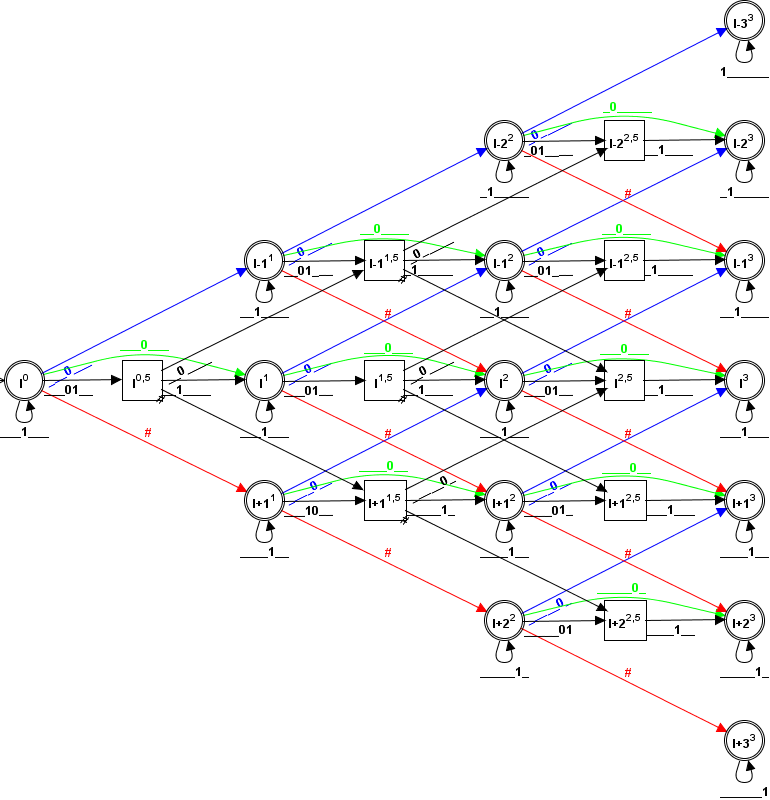
\includegraphics[width=\linewidth,height=\textheight,keepaspectratio]{pic/automata/unidamerau}%
\caption{Der Versuch eines universellen Damerau-Levenshtein-Automaten für den Abstand 3. Die rechteckigen Zustände sind die zusätzlichen Zustände zum Levenshtein-Automaten. Die farbigen Zustände sind die Zustände aus dem Levenshtein-Automaten (rot Löschen, blau Einfügen, grün Substitution). Die schwarzen Übergänge sind die zusätzlich benötigten Übergänge. Der waagerechte Übergang durch den zusätzlichen Zustand ist ein normaler Tausch, der steigende ein zusätzliches Einfügen, der fallende ein zusätzliches Löschen.}%
\end{figure}
\section{Vergleich zu Mihov/Schulz}
Die grundsätzliche Funktionsweise des hier vorgestellten Levenshteinautomaten ist die gleiche wie bei Mihov/Schulz. Es gibt jedoch ein paar Unterschiede. Mihov/Schulz benutzt eine getrennte Nicht-Endzustands- und Endzustandsmenge, sie erweitern also am Ende die symbolischen Dreiecke nicht um virtuelle Zustände. Entsprechend werden in der Kodierung, wenn das Muster zu Ende ist, keine Dummy-Symbole eingefügt, sondern der charakteristische Vektor wird kürzer. Die Anzahl der charakteristischen Vektoren ist hier genau die Länge der Eingabe. Dieses Vorgehen macht es allerdings nötig, den charakteristischen Vektor um eine Stelle zu erweitern. Diese Stelle wird benutzt, um zu überprüfen, ob das Ende der Eingabe erreicht ist, denn wenn der charakteristische Vektor nicht mehr vollständig ist, wird in die Endzustandsmenge gewechselt.

Das bedeutet, dass der Mihov/Schulz-Automat eine größere Zustandsmenge hat (mehr als die Hälfte kommt nochmal dazu) und eine andere Eingabewortlänge. Auf der einen Seite wird pro Vektor ein Zeichen mehr benötigt, auf der anderen Seite werden die Vektoren am Ende kürzer. Es kann außerdem sein, dass bei der hier vorgestellten Methode mehr charakteristische Vektoren berechnet werden müssen. Allerdings ist eine konstante Blockgröße vorteilhaft bei der Simulation. Große Abweichungen der Wortlänge (also größer als der Abstand) kann bereits bei der Kodierung abgefangen werden, da diese Wörter nicht akzeptiert werden können. Das gleicht den großen Unterschied der Eingabegrößen bei kurzer Eingabe zu einem langen Muster aus.

Außerdem wurde bei Mihov/Schulz direkt ein DEA konstruiert ohne den Zwischenschritt über den NEA. Dabei betrachten sie direkt eine optimierte Potenzmenge der Zustände in dem symbolischen Dreieck, was genau den Zuständen entspricht, die die Potenzmengenkonstruktion bei den Übergängen mit geforderter 0 berechnet. Die Potenzmenge wird optimiert, indem geschaut wird, ob von mehreren Zuständen mit gleicher Eingabe ein Endzustand erreicht werden kann. Diese müssen dann nicht gesondert betrachtet werden. Die Zustände, die so zusammengefasst werden können, sind genau die, die in einem symbolischen Dreieck liegen; diese Zustände können dann durch den Zustand in der Spitze repräsentiert werden.

Die Konstruktion der Übergangsfunktion wird nicht explizit beschrieben. Es wird lediglich erklärt, dass die Übergänge so gebaut werden müssen, dass die aktiven Zustände für die Berechnungen übereinstimmen müssen. Das bedeutet, dass bei den Übergängen innerhalb einer Fehlerstufe an den signifikanten Stellen des Zielzustandes eine 1 stehen muss, und an den Stellen, die zwar signifikante Stellen des Start- aber nicht des Zielzustandes sind, eine 0 stehen muss. Für Übergänge von einer Fehlerstufe auf die nächste, gibt es zwei Übergänge, nämlich mit 01 an der signifikanten Stelle des Startzustandes zu dem Zustand mit den signifikanten Stellen -1, +0 und +1 relativ zur alten signifikanten Stelle und einen mit 00 an der signifikanten Stelle zum Zustand ohne die signifikante Stelle +1.

\begin{figure}[htbp]
\centering
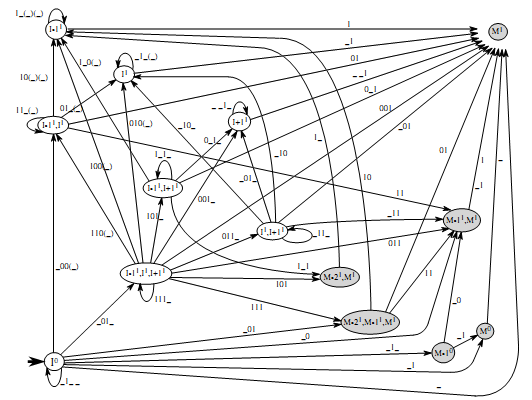
\includegraphics{pic/automata/unidlevenshteinmihov}%
\caption{Deterministischer universeller Levenshtein-Automaten für den Abstand 1 nach Mihov/Schulz aus \cite{lit01}}%
\end{figure}
\endinput
